\documentclass {CSEThesis}
% Standard packages
\usepackage{amsmath}        % Extra math definitions
\usepackage{graphics}       % PostScript figures
\usepackage{setspace}       % 1.5 spacing
%\usepackage{psfig,epsfig}
\usepackage{multicol}
\usepackage{subfigure}
\usepackage{hyperref}
\usepackage{epsfig,color}
% Custom packages
%\usepackage[first]{datestamp}   % Datestamp on first page of each chapter
\usepackage{caption}
\usepackage{amsmath}
\usepackage{breqn}
\usepackage{color}
%===== page layout
% Define the side margins for a right-side page
%\insidemargin = 1.3in \outsidemargin = 0.9in
% Above margin is space above the header
% Below margin is space below footer
%\abovemargin = 1.5in \belowmargin = 0.05in


\btptitle = {AI in Image Processing} % { and } are needed around your name
\name = {Kaushal Kishore}          % and other feilds. don't remove.
\rollno = {111601008}
\email = {111601008@smail.iitpkd.ac.in}
\guide = {Dr. Chandra Shekar}


\begin{document}

\begin{titlepage}
\begin{center}
\textheight 15.5in \textwidth 12.5in {\large\sf  \textbf{\the\btptitle}}\\[12ex]
{\small{\textsl{ \textbf{A Project Report Submitted \\
in Partial Fulfillment of the Requirements \\
for the Degree of \\
[3ex]\small \bf Bachelor of Technology}}}}\\
[16ex] \emph{by}
\\[2ex]
{\sf \sf \textbf{\the\name}\\
             (\the\rollno)}\\[1ex]
\emph{under the guidance of}\\[2ex]
{\sf \bf \the\guide} \\[7ex]

\vspace{1.2in}

 \begin{figure}[!h]
\centering
 
\includegraphics[width=0.15\textwidth]{IITPkdFullLogoColor}
 \end{figure}



{\small\bf DEPARTMENT OF COMPUTER SCIENCE AND ENGINEERING}  \\[1ex]
%{\small \bf{INDIAN INSTITUTE OF TECHNOLOGY PALAKKAD}}
%\\[2ex]
%
%  {\color{red} \hrule height 0.5ex}
% \vskip 1ex
% May \the\year 
\end{center}
\end{titlepage}



\raggedbottom
\doublespacing
\pagenumbering{roman}
\chapter*{\centering \underline{CERTIFICATE}}
\vskip 2ex \emph{\quad This is to certify that the work contained
in this thesis entitled ``\textbf{\the\btptitle}'' 
is a bonafide work of \textbf{\the\name}
(\textbf{Roll No. \the\rollno}), carried out in the Department of
Computer Science and Engineering, Indian Institute of Technology
Palakkad under my supervision and that it has not been submitted
elsewhere for a degree.} \vskip 15ex

\begin{flushright}
	\textbf{Dr. Chandra Shekar}\\
	Assistant Professor \\
	Department of Computer Science \& Engineering \\
	Indian Institute of Technology Palakkad
\end{flushright}
\hfill 
\hfill 






\chapter*{\centering Acknowledgements}
\quad Write acknowledgements, if your want to.



\tableofcontents 

\addcontentsline{toc}{chapter}{List of Figures} 
\listoffigures 

\addcontentsline{toc}{chapter}{List of Tables} 
\listoftables

\pagenumbering{arabic}
\def\headrulehook{\color{black}}      % Color the header rule

%========== Chapters
\typeout{}
\chapter{Introduction}
\pagenumbering{arabic}\hspace{3mm}

Image processing libraries these days (eg. Open CV) uses the conventional methods which have the possibility to be outperformed by methods which leverage the power of artificial intelligence. Some recent research have shown that some of these AI based methods are able to perform atleast as good as conventional approaches. The aim of this project is to implement, apply and possibly improve upon the existing approaches in Digital Image Processing and Computer Vision. These common tasks can include (not limited to) applications like: Image Compression, Denoising, Super Resolution, Flow Estimation, Object Detection, etc.


\section{Image Processing}

\begin{figure}[!ht]
    \centering
    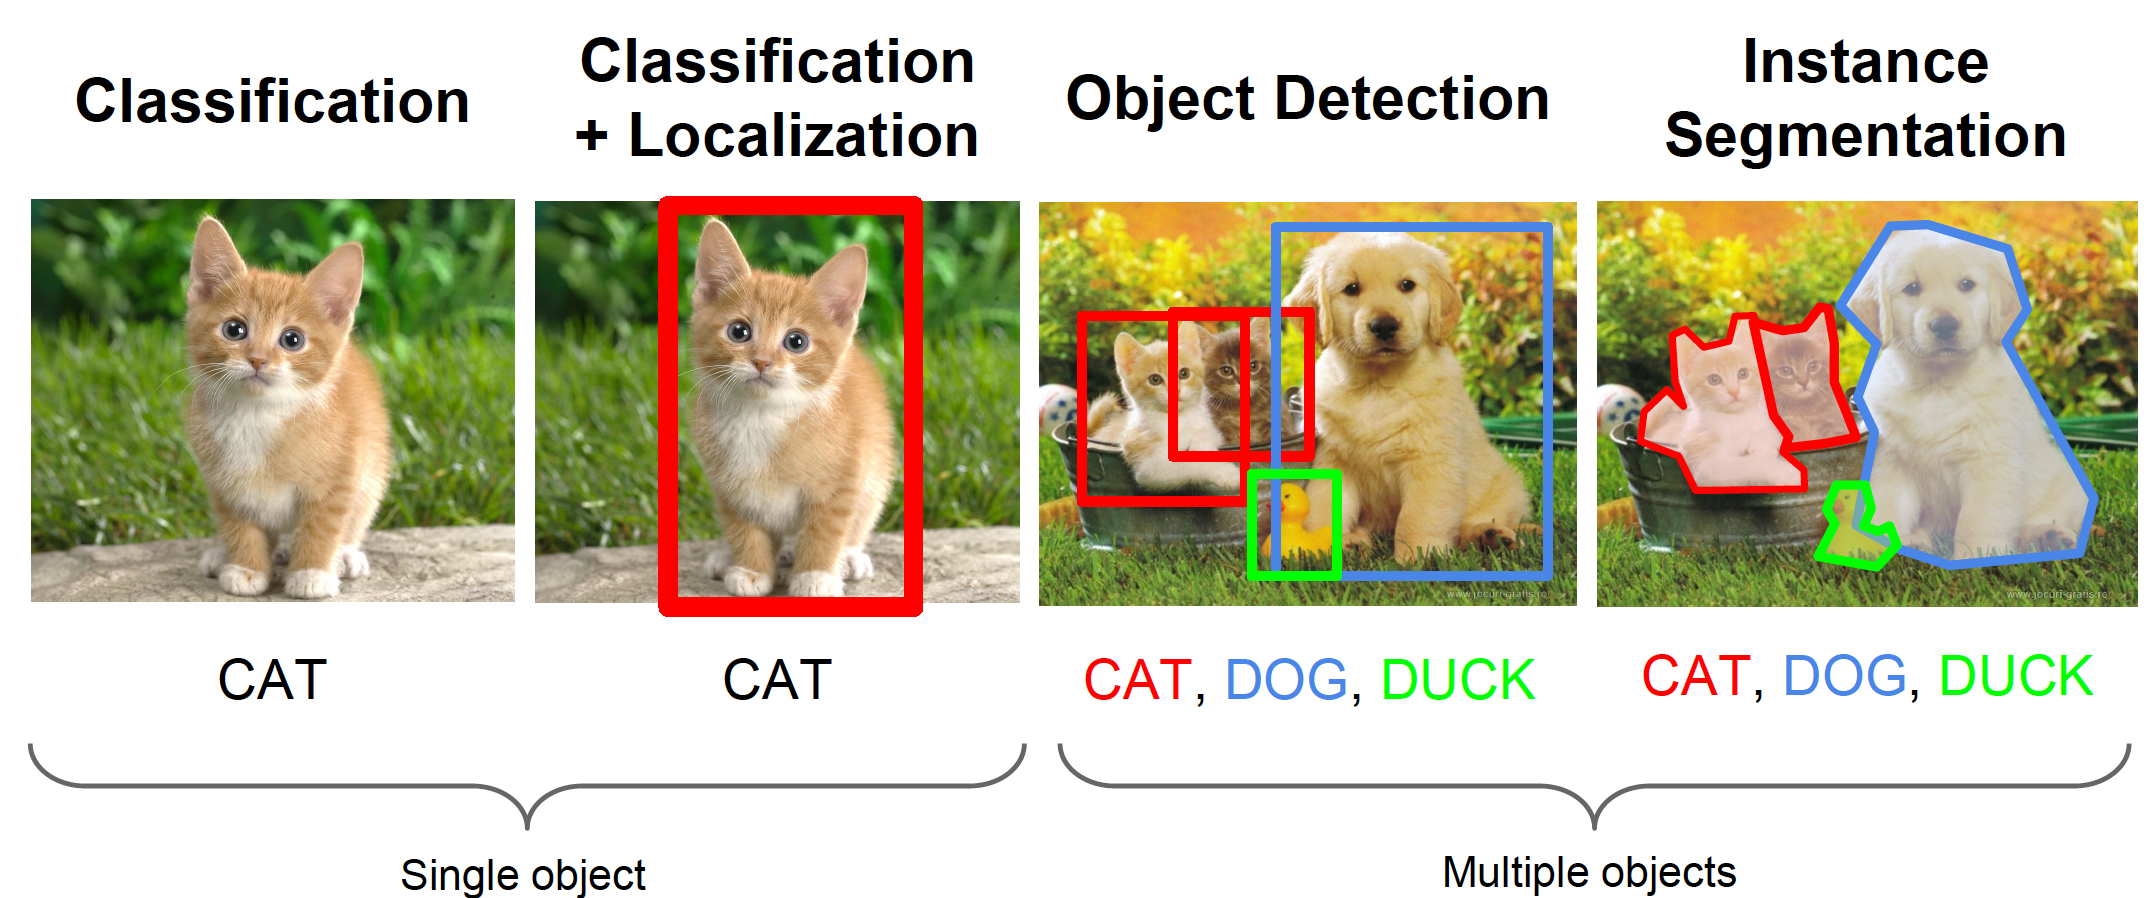
\includegraphics[width=0.75\textwidth]{fig/1-1.png}
    \captionsource{Examples of pattern recognition}
    {\href{https://www.cs.cornell.edu/courses/cs4670/2016sp/lectures/lec41_recowrapup_web.pdf}{www.cs.cornell.edu}}
    \label{fig:exPatternRecognition}
\end{figure}

Image processing is manipulating an image in order to enhance it or extract information from it. It is widely useed in medical visualization, biometrics, self-driving vehicles, gaming, surveillance, and law enforcement. It can used in various ways: visualization, restoration, imformation retrieval, pattern recognition, etc.

General approach of image processing involves eight key phases: image acquisition, image enhancement, image restoration, color space transformation, compression or decompression, morphological processing, recognition, and representation. It is very difficult to carry out these steps manually on a very big data, this is where AI and ML algorithms become very helpful.

\begin{figure}[!ht]
    \centering
    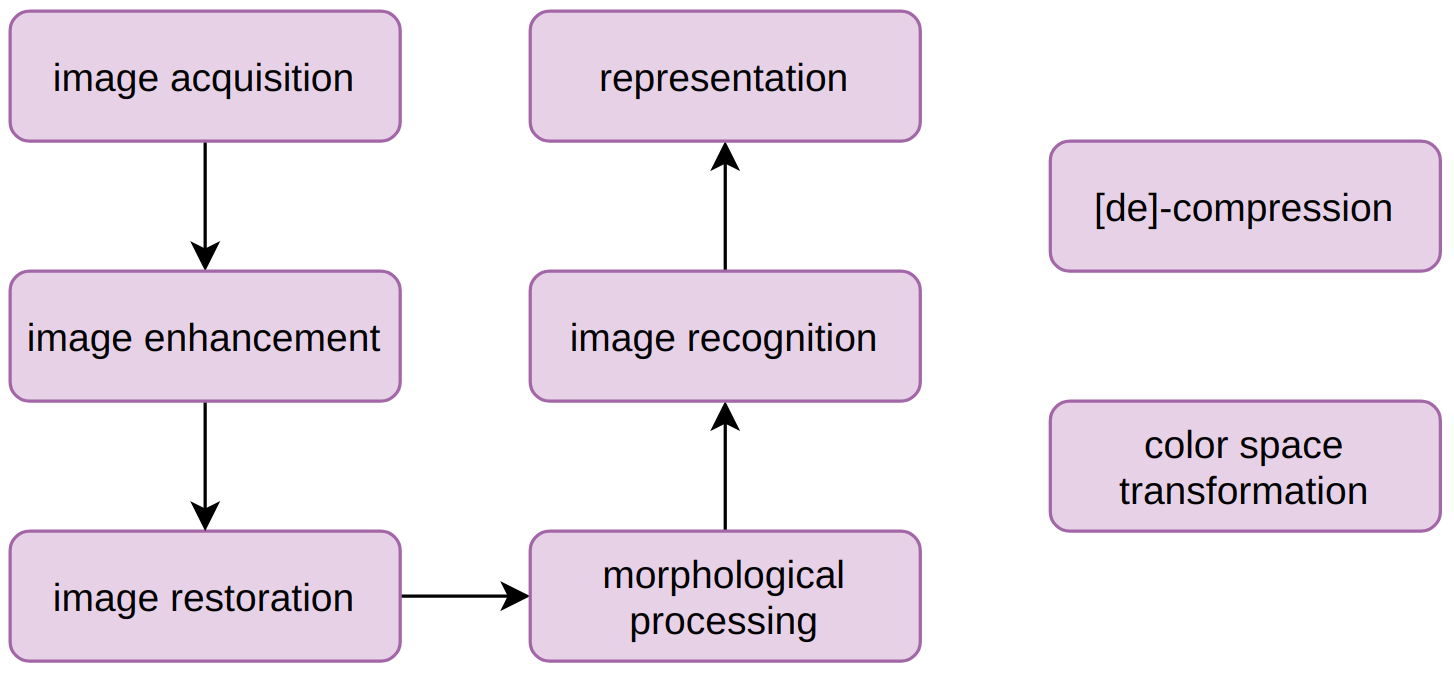
\includegraphics[width=0.75\textwidth]{fig/1-2.png}
    \caption{Key phases of image processing}
    \label{fig:keyPhasesOfImageProcessing}
\end{figure}

\section{Recent advances}

Modern AI algorithms have enabled computer to perform detection, segmentation, recognition, compression, extraction, generation, and discrimination. Every year a state of the art model is invented to solve the existing problem in a better way. It is now an established fact that machines are now better than humans in counting, classifying and segmenting instances. 

\cleardoublepage 
\typeout{}
\chapter{Image Compression}

A data compression algorithm transforms the data to occupy a less space. The original data is encoded by a program called encoder, to a compressed representation using a fewer number of bits. Decoder is responsible for decompressing the compressed representation. 

\begin{figure}[!ht]
    \centering
    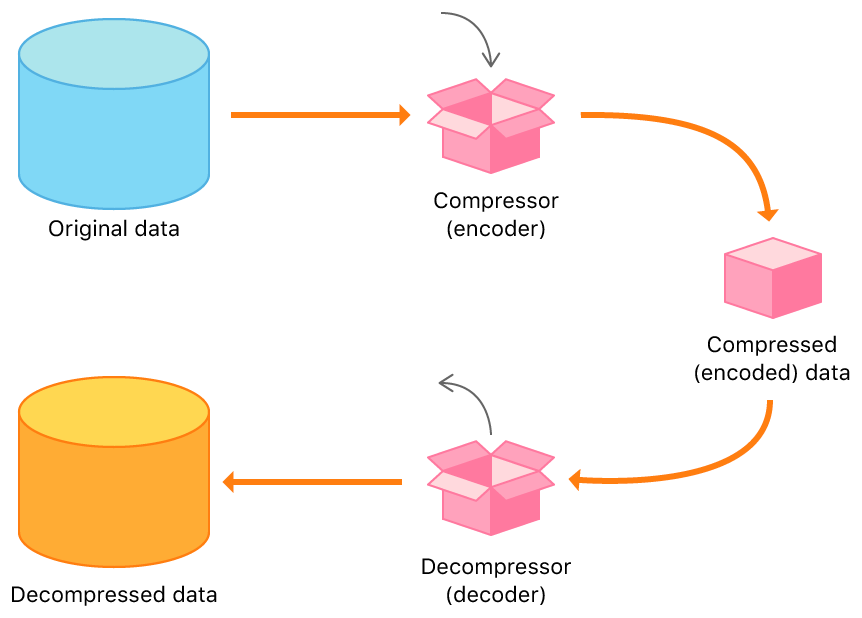
\includegraphics[width=0.50\textwidth]{fig/2-1.png}
    \captionsource{Compression phases}
    {\url{https://developer.apple.com/documentation/compression}}
    \label{fig:phasesCompression}
\end{figure}

Image compression is very crucial in order to reduce the size of disk space used as well as reduce the amount of internet bandwidth used while loading images. It’s also important to compress images for people accessing the internet via low bandwidth connections.

\section{Lossy vs. Lossless}

The compression technique where the decompressed data is exactly same as original data is called as lossless compression otherwise it is known as lossy compression technique because some information is lost during coding-encoding phase. Two well-known codecs for image compression are JPEG and PNG. PNG is lossless and JPEG is lossy.

\vspace{2em}

\begingroup
\centering
    \begin{tabular}{ | p{7cm} | p{7cm} | }
    \hline
    Lossy & Lossless \\ \hline
    A compression
    that permits reconstruction only of an approximation of the original data, though usually with an improved compression rate. & A class of data compression that allows the original data to be perfectly reconstructed from the compressed data. \\ \hline
    Reduces the quality. & Does not reduce the quality. \\ \hline
    Data reduction is higher. & Data reduction is lower. \\ \hline
    Commonly used to compress multimedia data such as audio (MP3), video and image (JPEG) files. & Used commonly for text, data files, etc. \\
    \hline
    \end{tabular}
\captionof{table}{Lossy vs Lossless}\label{tbl:lossyvslossless}
\endgroup


\section{Dimensionality Reduction PCA}

Principal components analysis (PCA) is one of a family of techniques for taking high-dimensional data, and using the dependencies between the variables to represent it in a more tractable, lower-dimensional form, without losing too much information. PCA is one of the simplest and most robust ways of doing such dimensionality reduction.

PCA is mathematically defined as an orthogonal linear transformation that transforms the data to a new coordinate system such that the greatest variance by some scalar projection of the data comes to lie on the first coordinate (called the first principal component), the second greatest variance on the second coordinate, and so on.


\begin{figure}[!ht]
    \centering
    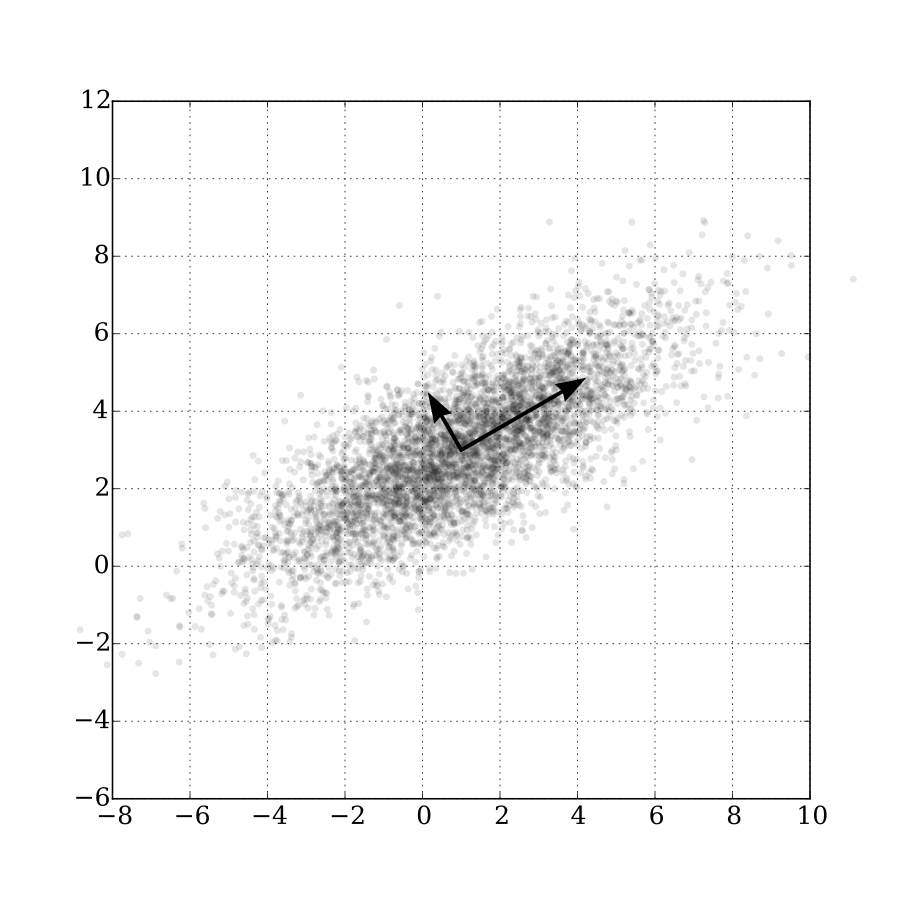
\includegraphics[width=0.65\textwidth]{fig/2-2.png}
    \captionsource{PCA of a multivariate Gaussian distribution centered at (1,3) with a standard deviation of 3 in roughly the (0.866, 0.5) direction and of 1 in the orthogonal direction.}
    {\url{https://en.wikipedia.org/wiki/Principal_component_analysis}}
    \label{fig:phasesCompression}
\end{figure}


Let $W$ be a $d \times d$ matrix whose columns are the principal components of $X$. The transformation $T = X W$ maps a data vector $x_{(i)}$ from an original space of $d$ variables to a new space of $d$ variables which are uncorrelated over the dataset. However, not all the principal components need to be kept. Keeping only the first $L$ principal components, produced by using only the first $L$ eigenvectors, gives the truncated transformation:

$T_L = XW_L$


where the matrix $T_L$ now has $n$ rows but only $L$ columns. In other words, PCA learns a linear transformation 
$t = W^{T}x, x \in \Re^{d}, t \in \Re^{L}$, where the columns of $d \times L$ matrix $W$ form an orthogonal basis for the $L$ features (the components of representation t) that are decorrelated. By construction, of all the transformed data matrices with only $L$ columns, this score matrix maximises the variance in the original data that has been preserved, while minimising the total squared reconstruction error $\left \| TW^T - T_LW_L^T\right \|_2^2 or \left \| X - X_L \right \|_2^2$.

The basic steps for computing the PCA is as follows:

\begin{enumerate}
    \item Standardize the d-dimensional dataset.
    \item Construct the covariance matrix.
    \item Decompose the covariance matrix into its eigenvectors and eigenvalues.
    \item Sort the eigenvalues by decreasing order to rank the corresponding eigenvectors.
    \item Select $L$ eigenvectors which correspond to the $L$ largest eigenvalues, where $L$ is the dimensionality of the new feature subspace $L \leq d$.
    \item Construct a projection matrix $W_L$ from the "top" $L$ eigenvectors.
    \item Transform the $d$-dimensional input dataset $X$ using the projection matrix $W_L$ to obtain the new $L$-dimensional feature subspace.
\end{enumerate}

\vspace{1em}

\begin{figure}[!ht]
    \centering
    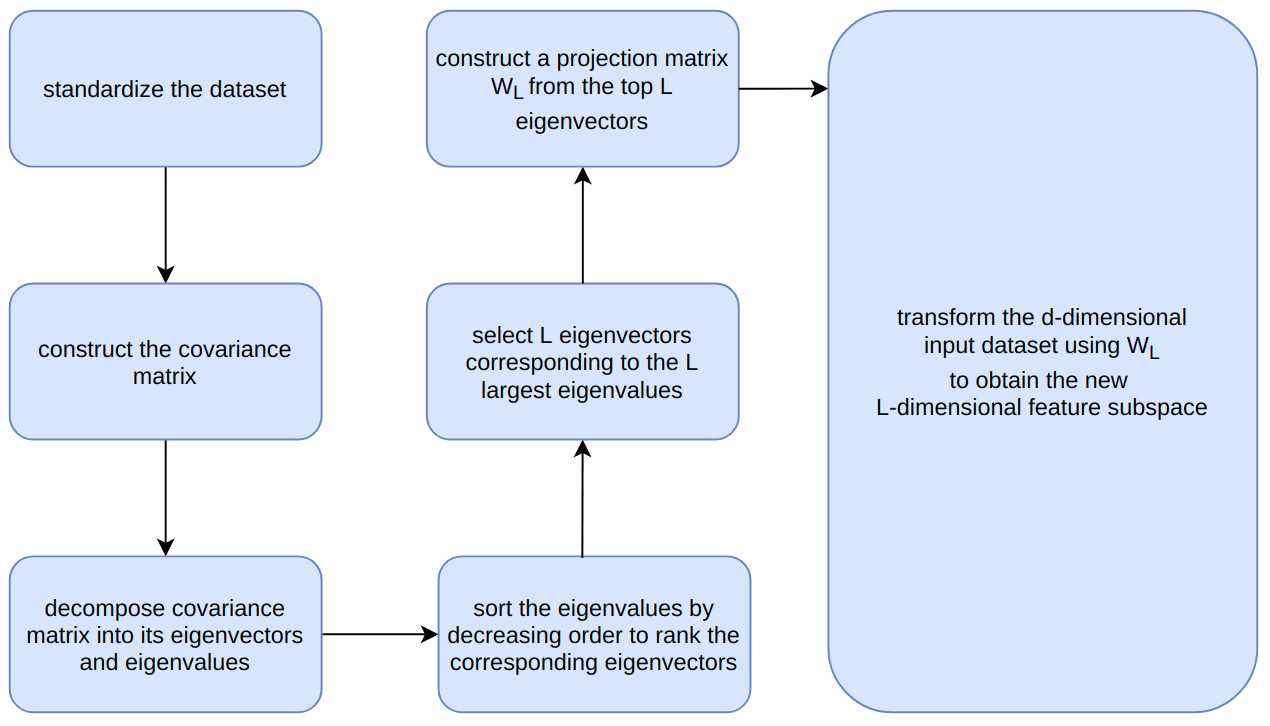
\includegraphics[width=0.75\textwidth]{fig/2-3.png}
    \caption{Steps for dimensionality reduction using PCA}
    \label{fig:dimensionalityReductionSteps}
\end{figure}

\vspace{1em}

\section{Image compression using PCA}

We will follow the steps mentioned in the previous section for dimensionality reduction using PCA. The results of the experiments are tabulated below:

\begin{figure}[!ht]
    \centering
    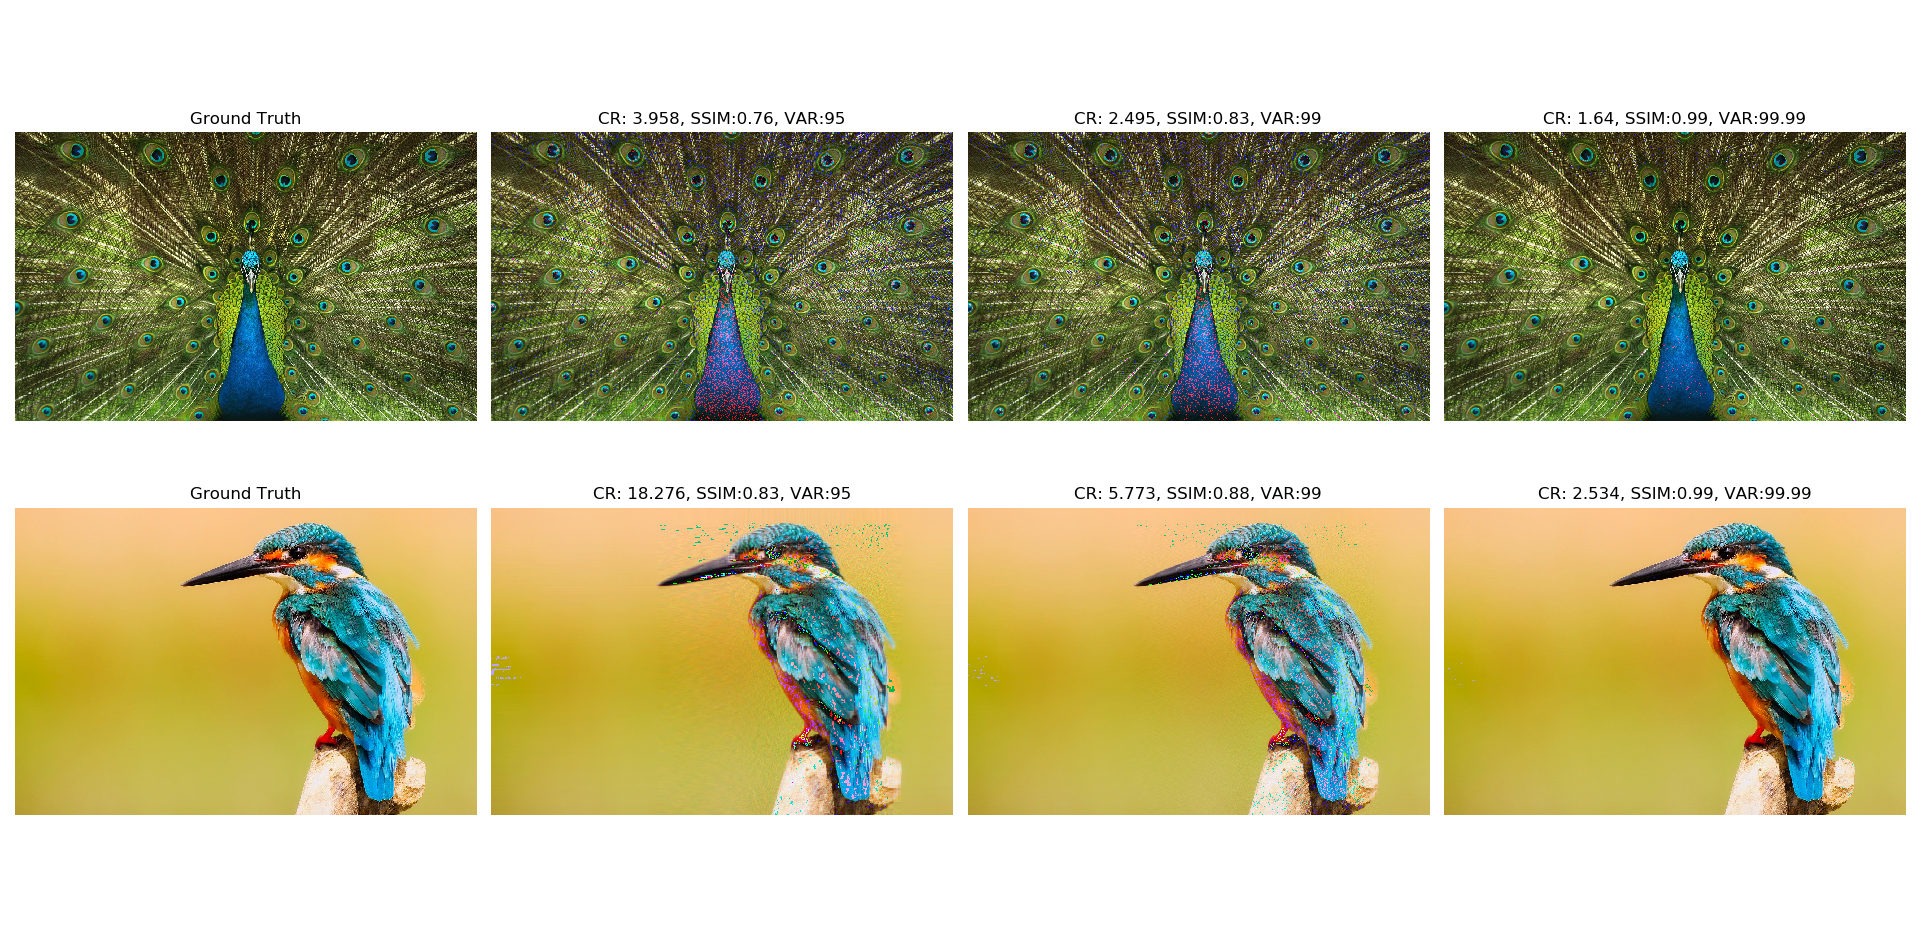
\includegraphics[width=1\textwidth]{fig/2-4.png}
    \caption{ CR = Compression Ratio, SSIM = Structural Similarity Index, VAR = Variance. Results of compression using the PCA method. Higher variance leads to more number of principal components and higher is the reconstructed image quality and lower the compression rate.}
    \label{fig:imageCompressionUsingPCA}
\end{figure}

Code for the above test can be found here: \href{https://github.com/KishoreKaushal/ImageCompression/tree/master/PCA}{@KishoreKaushal/ImageCompression/}

It is clear from the above experiment that higher variance leads to more number of principal components and higher is the reconstructed image quality and lower the compression rate. Infact, the first $L$ principal components is selected to get atleast the given number of variance.
\cleardoublepage 
\typeout{}
\chapter{JPEG}

\section{Overview}

JPEG, which stands for Joint Photographic Experts Group (the name of the committee that created the JPEG standard) is a lossy compression algorithm for images. A lossy compression scheme is a way to inexactly represent the data in the image, such that less memory is used yet the data appears to be very similar. This is why JPEG images look almost the same as the original images they were derived from most of the time unless the quality is reduced significantly, in which case there will be visible differences.

The JPEG algorithm takes advantage of the fact that humans can't see colors at high frequencies. These high frequencies are the data points in the image that are eliminated during the compression. JPEG compression also works best on images with smooth colour transitions.

JPEG is a commonly used method of lossy compression for digital
images. The degree of compression can be adjusted, allowing a
the tradeoff between storage size and image quality with a
compression ratio 10:1 but with little perceptible loss in image
quality.

\begin{figure}[!ht]
    \centering
    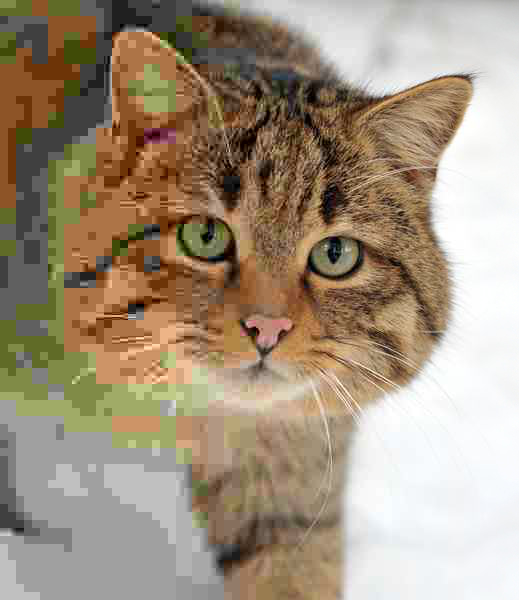
\includegraphics[width=0.40\textwidth]{fig/3-1.png}
    \captionsource{A photo of a European wildcat with the compression rate decreasing and hence quality increasing, from left to right.}
    {\url{https://en.wikipedia.org/wiki/JPEG}}
    \label{fig:jpegCompression}
\end{figure}

\vspace{2em}

\section{Algorithm}

\begin{figure}[!ht]
    \centering
    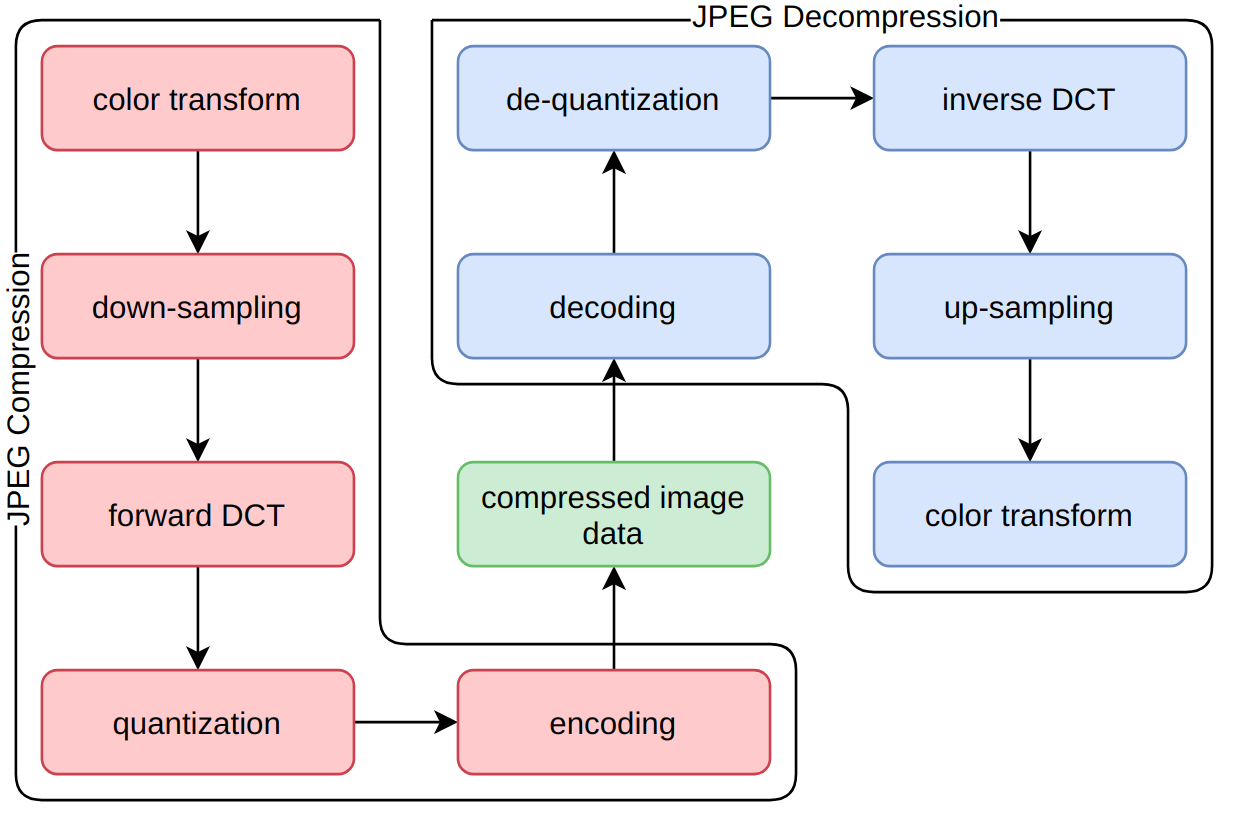
\includegraphics[width=0.80\textwidth]{fig/3-2.png}
    \caption{JPEG Schematic}
    \label{fig:jpegSchematic}
\end{figure}


\subsection{Splitting}

JPEG uses transform coding, it is largely based on the following observations:

\begin{itemize}
    \item Usually image contents change relatively slowly across images, i.e., it is unusual for intensity values to alter up and down several times in a small area, for example, within an $8 \times 8$ image block. A translation of this fact into the spatial frequency domain, implies, generally, lower spatial  frequency components contain more information than the high frequency components which often correspond to less useful details and noises.
    \item Experiments suggest that humans are more immune to loss of higher spatial frequency components than loss of lower frequency components. Human vision is insensitive to high frequency components.
\end{itemize}

Hence, first step is to split the image into $8 \times 8$ blocks non-overlapping pixel blocks. If the image cannot be divided into $8 \times 8$ blocks then the block is zero padded.

\vspace{1em}

\begin{figure}[!ht]
    \centering
    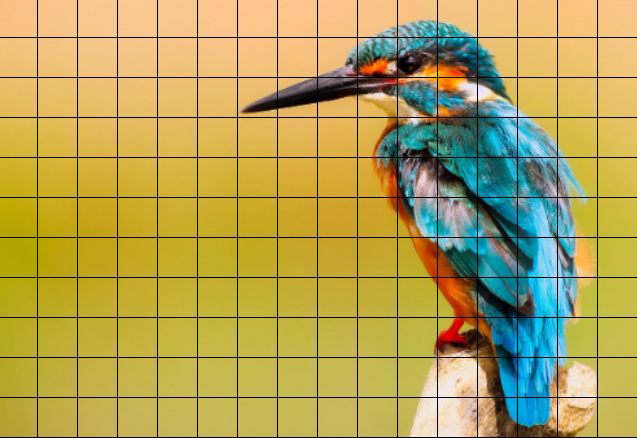
\includegraphics[width=0.50\textwidth]{fig/3-3.png}
    \caption{Splitting into $8 \times 8$ blocks}
    \label{fig:splitting}
\end{figure}

\subsection{Color Space Transform}

JPEG makes use of $[Y, Cb, Cr]$ model instead of $[R, G, B]$ model. There is a reason for using the color space. The human eye is more sensitive to luminance than to chrominance. 

\begingroup
\centering
    \begin{tabular}{|l|}
    \hline
    $Y = 0.299R + 0.587G + 0.114B$              \\ \hline
    $Cb = -0.1687R - 0.3313G + 0.5B + 128$      \\ \hline
    $Cr = 0.5R - 0.4187G - 0.0813B + 128$       \\ \hline
    $R = Y + 1.402 (Cr - 128)$                   \\ \hline
    $G = Y - 0.34414 (Cb - 128) - 0.71414(Cr - 128)$ \\ \hline
    $B = Y + 1.772  (Cb - 128)$                   \\ \hline
    \end{tabular}
\captionof{table}{RGB and YCbCr conversion table}\label{tbl:RGBYCbCrTable}
\endgroup


\subsection{Down-sampling}

After the color space transformation, the image is downsampled.
Downsampling happens in such a way that $Y$ is taken for each pixel whereas $Cb$ and $Cr$ is taken for $2 \times 2$ blocks.

Sometimes this steps is not carried out.

\subsection{Discrete Cosine Transform}

The key to the JPEG baseline compression process is a mathematical transformation known as the Discrete Cosine Transform (DCT). The DCT is in a class of mathematical operations that includes the well known Fast Fourier Transform (FFT), as well as many others. The basic purpose of these operations is to take a signal and transform it from one type of representation to another. For example, an image is a two-dimensional signal that is perceived by the human visual system. The DCT can be used to convert the signal (spatial information) into numeric data (“frequency” or “spectral” information) so that the image's information exists in a quantitative form that can be manipulated for compression.



\section{Conclusion}
In this chapter, we proposed a distributed algorithm
for construction of xyz.
The complexity of this algorithm is $O(n \log n)$.
Next chapter presents
another distributed algorithm which has linear time 
complexity based on xyz.


\cleardoublepage 
\typeout{}
\chapter{Perceptual Image Compression}

Prakash2017 \cite{Prakash2017} introduced a powerful CNN
tailored to the specific task of semantic image understanding to achieve higher visual quality in lossy compression. A modest increase in complexity is incorporated into the encoder which allows a standard, off-the-shelf jpeg decoder to be used. While JPEG encoding may be optimized for generic images, the process is ultimately unaware of the specific content of the image to be compressed. This technique makes JPEG content-aware by designing and training a model to identify multiple semantic regions in a given image.


\section{Content aware compression}

The existing compression standards are content unware. For example, consider the case of JPEG algorithm, during the quantization step the quantization tables that are used are experimentally decided on a well-established theory that humans are insensitive to chrominance in contrast to luminance. An obvious question is can't we have a quantization table tailored specifically for each image. Of course, determining this table manually is a very uncertain and difficult task, and its well suited for the machine to do this for us.

The idea here is to locate multiple regions of interest (ROI) within a single image and noting the fact that it's not an object detection problem and hence the precision of the boundary doesn't matter. Also, the model needs to learn a single class-invariant feature map by learning separate feature maps for each of a set of object classes and then summing over the top features.

\section{Conclusion}
In this chapter, we proposed another distributed algorithm for
XYZ. This algorithm has both time complexity of $O(n)$ where $n$
is the total number of nodes.  In next chapter, we conclude and
discuss some of the future aspects.


\cleardoublepage 
\typeout{}
\chapter{Conclusion and Future Work}

write results of your thesis and future work.


\typeout{}

\bibliographystyle{IEEEtran}
\bibliography{btp}
\end{document}

